%   PACKAGES AND CUSTOMIzATIONS  %%%%%%%%%%%%%%%%%%%%%%%%
\documentclass[12pt]{article}
\usepackage{amsmath}
\usepackage{amssymb}
\usepackage{amsthm}
\usepackage[pdfborder={0 0 0}]{hyperref}
\usepackage{graphicx}
\usepackage{caption}
\usepackage{natbib}
\usepackage{wrapfig}
\usepackage{enumitem}
\setlist[enumerate]{itemsep=0mm}
\usepackage{multirow}
\usepackage{lscape}
\usepackage{caption}
\usepackage{subcaption}
\usepackage{float}
\usepackage{hyperref}
\usepackage{tabularx}
\usepackage{rotating}
\captionsetup[subfigure]{position=top, labelfont=bf,textfont=normalfont,singlelinecheck=off,justification=raggedright}
\renewcommand{\vector}[1]{\mathbf{#1}}
\usepackage{adjustbox}
\usepackage{bm}


\newcommand{\transectAbb}{Data for each glacier are divided into lower hourglass (LH), lower circle (LC), lower midline (LM), upper hourglass (UH), upper circle (UC), upper midline (UM), and upper transect (UT).}
\newcommand{\params}{Topographic parameters are distance from centreline ($d_C$), elevation ($z$), aspect ($\alpha$), slope ($m$), northness ($N$), curvature ($\kappa$), and Sx. }
\newcommand{\boxplot}{Within each box, the mean is shown as a circle, the median as a horizontal line, the interquartile range (IQR) as a coloured box, two times the IQR as dashed lines beyond the box, and outliers as single points. }
\newcommand{\boxMatlab}{Red line indicates median, blue box shows first quantiles, bars indicate minimum and maximum values (excluding outliers), and red crosses show outliers, which are defined as being outside of the range of 1.5 times the quartiles (approximately $\pm2.7\sigma$). }
\newcommand{\topomap}{Arrows indicate glacier flow direction and black dots show snow depth sampling locations. }
\newcommand{\swedots}{Observed SWE values are overlain on the maps. }


\begin{document}

\section{Kriging}
\label{sec:kriging}

\subsection{Background}

Physical surfaces vary continuously and must therefore be spatially correlated at short distance but statistically independent at large distances \citep{Davis1986}. If sampling points are distributed throughout a surface, the degree of spatial correlation of the observed surface can be determined and the surface can then be interpolated between sampling points. Kriging is a geostatistical interpolation method that finds a set of optimal weights for the values at each sampling location based on the spatial correlation of measured values and then estimates values at unsampled locations \citep{Davis1986, Li2014}. The kriging estimate ($\hat{z}$) at point $x_0$ is found using the equation
\begin{equation}
\label{eq:kriging}
\hat{z}(x_0) - \mu = \sum_{i=1}^{n} \lambda_i [z(x_i)-\mu(x_0)],
\end{equation}
where $\mu$ is a known stationary mean, $\lambda_i$ is a kriging weight, $z(x_i)$ is the measured value of the surface at point $x_i$, $n$ is the number of sampled points used to make the estimation (depends on size of sampling window), and $\mu(x_0)$ is the mean value of sampled points in the search window \citep{Wackernagel2003, Li2008}. Slight variations on Equation \ref{eq:kriging} result in various forms of kriging that are suited for different data sets. The kriging weights are estimated by minimizing the variance or the squared error, which is given by
\begin{align}
\mathrm{var}[\hat{z}(x_0)] &= E[(\hat{z}(x_0)-z(x_0)^2)]\\
&=\sum_{i=1}^{n}\sum_{j=1}^{n}\lambda_i \lambda_j C(x_i-x_j)+C(x_0-x_0)-2 \sum_{i=1}^{n} \lambda_i C(x_i-x_0),
\end{align}
where $C(x_i-x_j) = \mathrm{Cov}[z(x_i),z(x_j)]$ is the covariance of the surface \citep{Li2008}. Kriging assumes that the variance does not depend on the sample location, but depends only on distance between samples.  Anisotropic kriging allows for variance to change with direction but the variance still does not depend on sample location. Isotropic variance was assumed in this study.

A physical surface is usually assumed to be noisy and this noise is captured by a ``nugget'' parameter that allows for the surface to vary smoothly and thus, not pass directly through each measured point. The nugget is a residual that encompasses sampling-error variance as well as the spatial variance at distances less than the minimum sample spacing \citep{Li2008}. Spatial correlation of data is estimated using imperical variance and is often plotted in the form of a variogram (see Section \ref{sec:variogram_intro}).  

There are many forms of kriging and each one is tailored to suit different data types (see \cite{Li2014}). The most appropriate type of kriging for this study is simple kriging. 

Simple kriging is used to estimate residuals about a constant and stationary mean $\mu$, which is typically calculated as the average of the data. Kriged estimates for simple kriging are found by slightly modifying Equation \ref{eq:kriging} to 
\begin{equation}
\hat{z}(x_0) = \sum_{i=1}^{n} \lambda_i z(x_i) +\left[1-\sum_{i=1}^{n} \lambda_i \right]\mu.
\end{equation}
Larger values of $\left[1-\sum_{i=1}^{n} \lambda_i \right]$ result in estimates that are closer to the data mean \citep{Li2008}. The value of $\left[1-\sum_{i=1}^{n} \lambda_i \right]$ generally increases in poorly sampled areas. 

\subsection{Methods}
\label{sec:kriging_methods}

Simple kriging is implemented using the R package \texttt{DiceKriging}, which approximates functions by first generating a kriging model from input data and then estimating data values at new locations based on their distance from observed data \citep{Roustant2012}. For the SWE data, a nugget value needs to be estimated by the \texttt{DiceKriging} package because the covariance length varies considerably over short distances. For this study, the kriged surface cannot not be estimated without a nugget, indicating that the function is not purely deterministic. Maximum likelihood is used to estimate both nugget and covariance values in \texttt{DiceKriging}. Negative values of kriged SWE were set to zero. For more details on implementation of \texttt{DiceKriging} see Appendix \ref{app:KrigingMethods}.

\subsection{Results}

There are large differences in spatial patterns of interpolated SWE distributions for the three study glaciers found using simple kriging (Figure \ref{fig:sweKRIGING}). The lower half of Glacier 4 has a relatively uniform SWE, while the accumulation area has both low and high values of SWE. The low density of sampling points in the accumulation area of Glacier 4 result in large gradients in SWE. Glacier 2 has two distinct and relatively uniform areas --- the lower ablation area has low SWE ($\sim$ 0.1 m w.e.) and the upper ablation and accumulation areas have higher SWE values ($\sim$ 0.6 m w.e.). The boundary between two these zones closely follows the outline of the ice dune area observed during field data collection. Glacier 13 does not appear to have any strong patterns and accumulation is generally low ($\sim$ 0.1--0.5 m w.e.). 

The glacier-wide winter mass balance on each glacier ($\mathrm{B_w}$), calculated as the mean SWE, that is found using simple kriging is considerably different to that found using a topographic regression (Figure \ref{fig:BMSmodelledSWE}). Accumulation on Glacier 4 is 0.09 m w.e. (15\%) higher and has larger spatial gradients in SWE when simple kriging is used. Conversely, simple kriging estimates are 0.13 m w.e. (23\%) and 0.08 m w.e. (22\%) lower for Glaciers 2 and 13, respectively, and the range of SWE values is smaller. The accumulation distribution estimated by simple kriging and by regression is qualitatively similar for Glacier 13 but differs considerably for Glacier 4 and 2. Glacier 4 has large SWE values in the accumulation area when simple kriging is used, which contrasts strongly with the mostly uniform accumulation estimated with regression. The converse is observed on Glacier 2, where the simple kriging estimate has a small SWE range and two distinct regions of SWE values while the regression estimate has a large range and a significant elevation gradient in accumulation. These spatial patterns highlight that kriging is sensitive to individual observation values in areas with sparse sampling. 

Estimates of the nugget found using maximum likelihood in the DiceKriging package also vary between glaciers (Table \ref{tab:sweKrigNugget}). Nugget values are small for both Glacier 2 and 13 ($\sim$ 0.004 m w.e.) and do not vary when different methods for interpolating snow density (Section \ref{sec:densityoptions}) are used. The nugget values for Glacier 4 are an order of magnitude larger and vary by $\sim$80\% of the minimum nugget value for this glacier. 

\begin{figure}
	\centering
	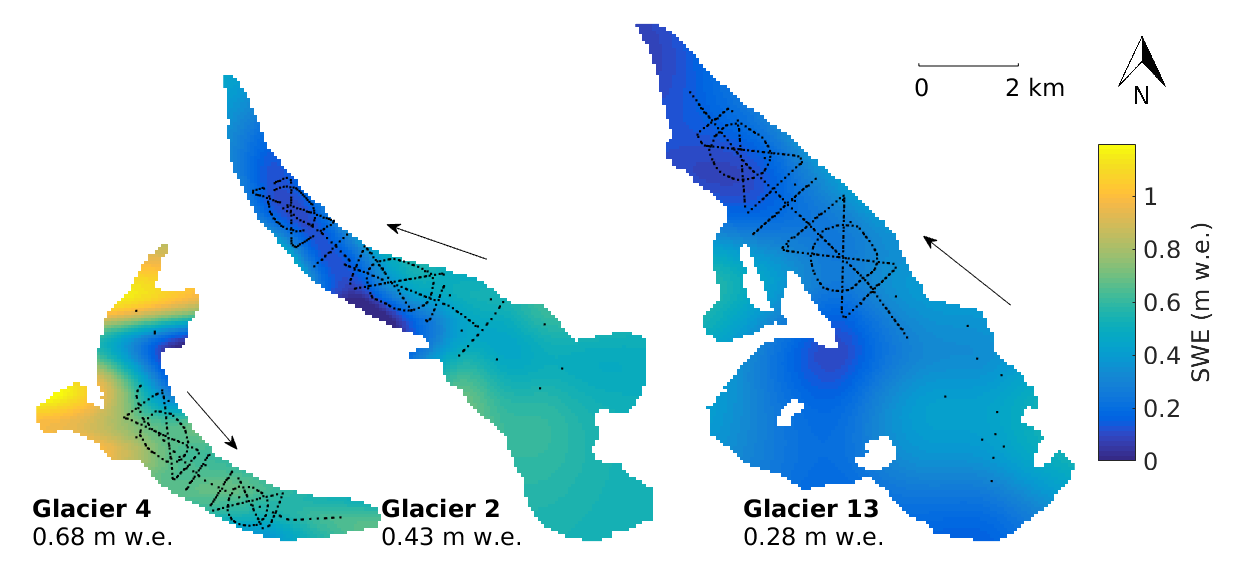
\includegraphics[width = \textwidth]{sweKriged.png}\\
	\caption{SWE distributions estimated by kriging. \topomap}
	\label{fig:sweKRIGING}
\end{figure}

\begin{table}[]
\centering
\caption{Nugget (m w.e.) values for SWE data with various snow density interpolation schemes estimated using maximum likelihood in DiceKriging package. S = Snowpit density values, F = Federal Sampler density values. See Section \ref{sec:densityoptions} for details on density options.}
\label{tab:sweKrigNugget}
\begin{tabular}{c|ccc}
\textbf{\begin{tabular}[c]{@{}c@{}}Density\\ Option\end{tabular}} & \textbf{Glacier 4} & \textbf{Glacier 2} & \textbf{Glacier 13} \\ \hline
\textbf{S1} & 0.015 & 0.004 & 0.004 \\
\textbf{F1} & 0.013 & 0.003 & 0.003 \\ \hline
\textbf{S2} & 0.009 & 0.004 & 0.004 \\
\textbf{F2} & 0.009 & 0.003 & 0.003 \\ \hline
\textbf{S3} & 0.016 & 0.004 & 0.005 \\
\textbf{F3} & 0.017 & 0.002 & 0.003 \\ \hline
\textbf{S4} & 0.014 & 0.004 & 0.004 \\
\textbf{F4} & 0.009 & 0.002 & 0.003
\end{tabular}
\end{table}

Comparing estimated and observed values of SWE (Figure \ref{fig:R2simplekrig}) shows that kriging is best able to predict SWE values on Glacier 2 and that kriging has the lowest predictive power on Glacier 4. This is similar to topographic regression estimates (Figure \ref{fig:BMSfit_opt8}), where the least variance was explained on Glacier 4 and the most variance was explained on Glacier 2. When compared to regression estimates, the R$^2$ values between SWE estimated using simple kriging and observed SWE are higher for all glaciers. Correlation values increase from 0.11, 0.63 and 0.36 to 0.25, 0.84 and 0.49 for Glaciers 4, 2 and 13, respectively. The largest difference in R$^2$ between these two methods is on Glacier 2, which also has the highest R$^2$ values. Note that the scatter of estimated and observed SWE values in Figure \ref{fig:R2simplekrig} is due to the nugget, which encompasses sampling-error variance and variance at distances smaller than the sample spacing.

\begin{figure}
	\makebox[\textwidth][c]{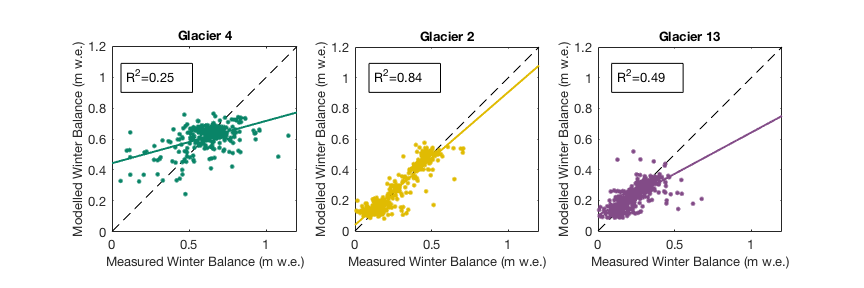
\includegraphics[width=1.2\textwidth]{krigSWEfit.png}}%
	\caption{Comparison of estimated (simple kriging) and observed (original) snow water equivalent (SWE) for three study glaciers. The SWE values were calculated using inverse-distance weighted snowpit densities (S4).}
	\label{fig:R2simplekrig}
\end{figure}

The confidence intervals for winter balance estimated using simple kriging are a large proportion of the estimated SWE values. The confidence interval range is at least half of the estimated SWE for all areas of the glacier, and in some areas, this proportion is more than four times the SWE estimate. The accumulation area, margin, and terminus of Glacier 2 all have especially high uncertainty. 

\begin{figure}[H]
	\centering
	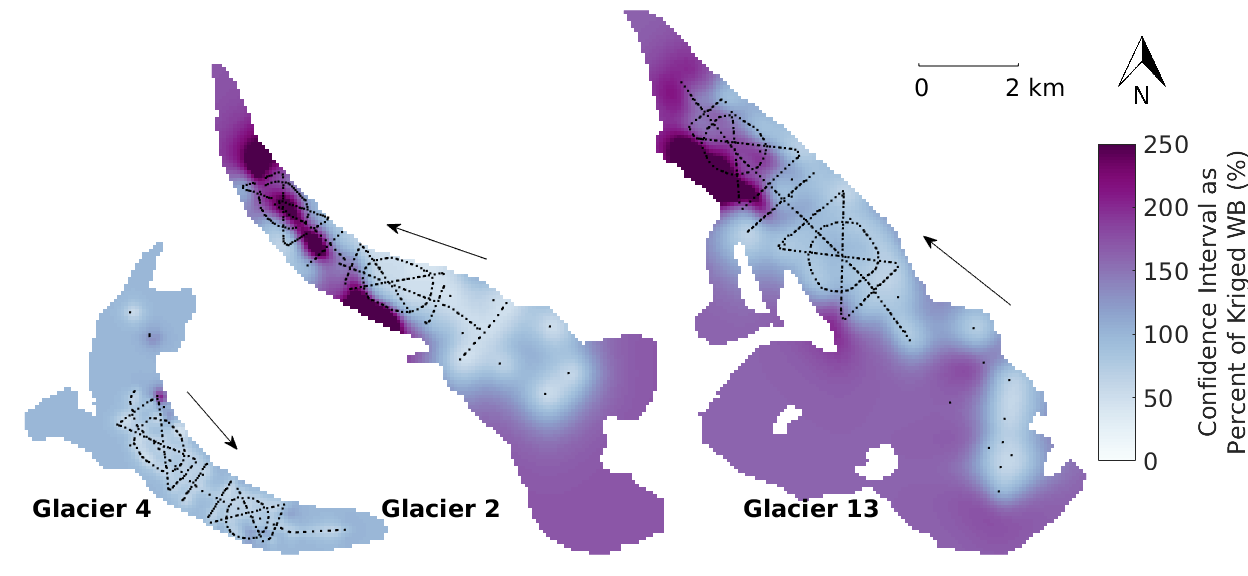
\includegraphics[width = \textwidth]{KrigingCI_percent.png}\\
	\caption{Simple-kriging winter-balance confidence interval (95\%) as a percent of distributed SWE, found using kriging. The SWE value were estimated using density S4. \topomap}
	\label{fig:Regression-Kriging}
\end{figure}

%%%
\section{Regression kriging}

\subsection{Background}

Regression kriging estimates values between measurement locations by combining a regression estimate (see Section \ref{sec:linearregression}) with a kriged estimate of the regression residuals (see Section \ref{sec:kriging}) \citep{Hengl2007}. First, the regression estimate is determined using auxiliary variables (e.g. terrain parameters such as elevation and slope). Then, simple kriging is used to interpolate regression residuals, which have and assumed mean of zero. The two surface estimates are then added. The final estimate can be written as 
\begin{align}
\hat{z}(x_0) &= \hat{m}(x_0) + \hat{e}(x_0)\\
& = \sum^p_{k=0}\hat{\beta}_k \cdot	q_k(x_0)+ \sum_{i=1}^{n} \lambda_i \cdot e(x_i),
\end{align}
where $\hat{m}(x_0)$ is the regression estimate and $\hat{e}(x_0)$ is the interpolated residual, $\hat{\beta}_k$ are the estimated regression coefficients, $q_k(x_0)$ are the regressors, $p$ is the number of regressors, $\lambda_i$ are the kriging weights for the residuals, and $e(x_i)$ is the residual at $x_i$.

Regression kriging can be thought of as an intermediate between pure kriging (no regression) and pure regression (small residuals) and can be more strongly skewed to either end-member based on the strength of the regression correlation \citep{Hengl2007}. Regression kriging is mathematically equivalent to universal kriging, in which auxiliary variables are used directly to determine the kriging weights \citep{Hengl2007}. However, separating the trend analysis and kriging steps has the advantage of being able to test regression methods that go beyond a basic linear trend. Kriging combined with regression has been found to produce better estimates of spatial fields when compared to simple kriging and co-kriging \citep{Knotters1995}.

\subsection{Methods}

First, SWE values are estimated with a regression of topographic parameters, as described in Section \ref{sec:linearregression}. The BMA regression is used for regression kriging because it resulted in a better fit than MLR between estimated and observed SWE. Second, the BMA residuals at each measurement location are calculated and the distributed residuals are found using simple kriging, as described in Section \ref{sec:kriging}. The BMA-estimated distributed SWE and kriging-estimated distrubuted residuals are then added together to obtain the final distributed winter balance. 

\subsection{Results}

The range, magnitude and spatial pattern of estimated regression residuals found using simple kriging varies between the three study glaciers (Figure \ref{fig:residualsKRIGING}). Generally, the range of residual values is highest on Glacier 4 and lowest on Glacier 13. Extreme values are located in the accumulation area of Glacier 4 with both strongly negative and strongly positive residuals located within a kilometre of each other. The low density of sampling points in the accumulation area biases the interpolation of residuals to fit the over- and underestimation of SWE at the two uppermost sampling locations. Residuals show less variation on Glacier 2, although relatively large residuals of approximately $\pm 0.4$ m w.e. are present in the upper ablation area along the ice margins. Glacier 13 has the smallest range of residuals but residual values are approximately equal to those of estimated SWE. The mean value of distributed residuals is positive for Glacier 4, indicating that the distributed residuals will increase the overall estimate of winter balance. Conversely, the mean residual for Glacier 2 is negative and will decrease the estimated winter balance. 

The winter balance found using simple kriging and regression kriging (Figure \ref{fig:Regression-Kriging}) shows a gradient in accumulation across the mountain range. Glacier 4 has the highest mean SWE and Glacier 13 has the lowest mean SWE. However, the accumulation gradient is steeper for simple kriged estimates than for regression kriged estimates. Glacier 4 has a similar mean SWE between the two methods but mean SWE on Glaciers 2 and 13 are much lower. All three glacier have the largest values of SWE in the upper part of the accumulation areas. 

SWE distribution estimated using regression kriging is similar to the winter balance estimated using topographic regressions for Glaciers 2 and 13 (Figure \ref{fig:Regression-Kriging}). The similarity is due to the relatively high explanatory power of the regressions, so the regression kriging estimate is closer to a pure regression. The distribution of SWE on Glacier 4 is more strongly affected by the kriged residuals because the regression had low explanatory power, resulting in larger residual values that changed the snow distribution, particularly in the accumulation area. The regression kriging for Glacier 4 is therefore closer to pure kriging.

Regression kriging produces the highest overall set of R$^2$ values (Figure \ref{fig:R2regressionkrig}). The correlation coefficient for Glacier 2 is especially high, with more than 80\% of the variance in observed SWE explained by the regression kriging model. Glacier 4 has the lowest correlation coefficient but this value is considerably higher than that of topographic regression or simple kriging. 

\begin{figure}[H]
	\centering
	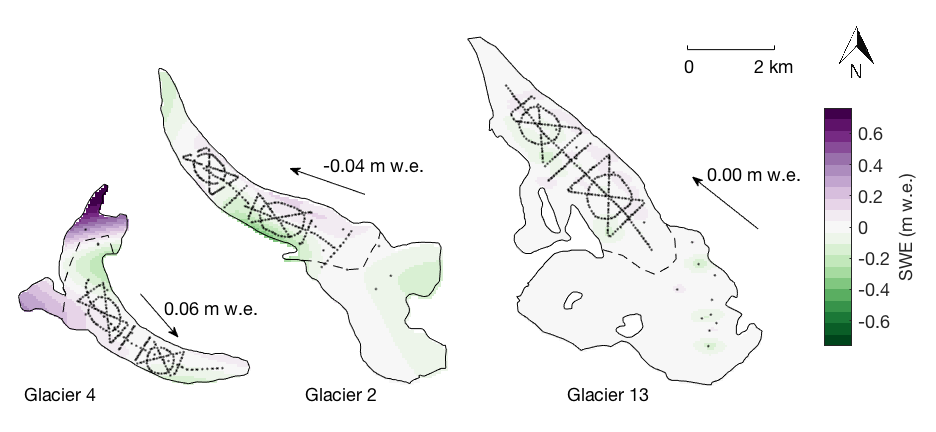
\includegraphics[width = \textwidth]{residualsKriged.png}\\
	\caption{Distributed BMA residuals estimated by simple kriging.  \topomap Dashed line indicates approximate ELA.}
	\label{fig:residualsKRIGING}
\end{figure}

\begin{figure}[H]
	\centering
	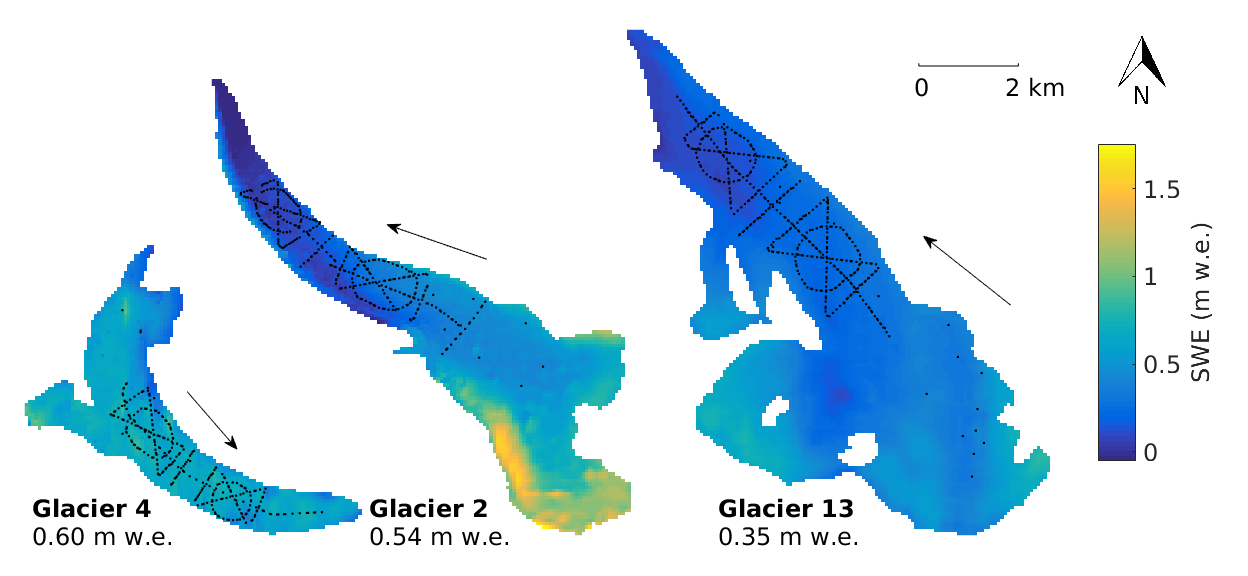
\includegraphics[width = \textwidth]{RegressionKriging.png}\\
	\caption{SWE distributions estimated by adding the kriged residuals to the SWE distributions estimated using topographic regression with BMA. \swedots Arrows indicate glacier flow direction.}
	\label{fig:Regression-Kriging}
\end{figure}

\begin{figure}[H]
	\makebox[\textwidth][c]{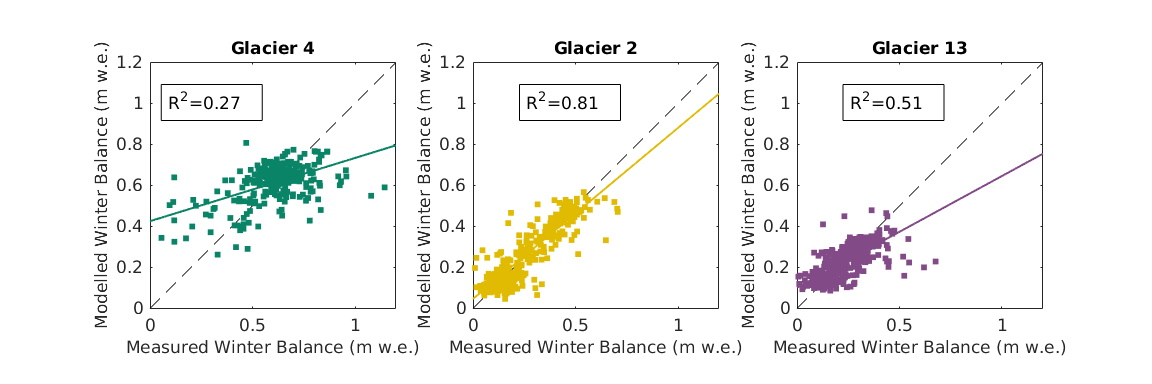
\includegraphics[width=1.2\textwidth]{krigRKfit.png}}%
	\caption{Comparison of estimated (regression kriging) and observed (original) snow water equivalent (SWE) for three study glaciers. The SWE values were calculated using inverse-distance weighted snowpit densities (S4).}
	\label{fig:R2regressionkrig}
\end{figure}


\section{Comparison of interpolation methods}

The choice of interpolation method affects the mean winter balance (Figure \ref{fig:InterpMethod_mean}). Kriging interpolation produces the highest mean value of SWE on Glacier 4. The estimates of SWE in the accumulation area are greatest when kriging is used because there is a single single high SWE value in the accumulation area. Kriging is sensitive to outliers in areas with sparse sampling. However, the winter balance is similar between interpolation methods and mean of observed data for Glacier 4. This similarity arises from the low correlation coefficient for all methods, resulting in values closer to the data mean. The observed SWE mean values for Glaciers 2 and 13 are much lower than the estimated winter balance. Both glacier show a significant correlation between SWE and elevation, so limiting sampling to the ablation area skewed the observed values of SWE to be lower than the mean. Relative differences in mean SWE between the three interpolation methods are similar for Glacier 2 and 13, with topographic regression producing the highest mean SWE and kriging producting the lowest. Kriging estimates lower SWE in the accumulation area of both glaciers because elevation is not incorporated into the model. A mountain range accumulation gradient exists when looking at the mean SWE values found using kriging and regression kriging, as well as in the observed data, but Glaciers 4 and 2 have the sample winter balance when topographic regression is used.

\begin{figure}
	\makebox[\textwidth][c]{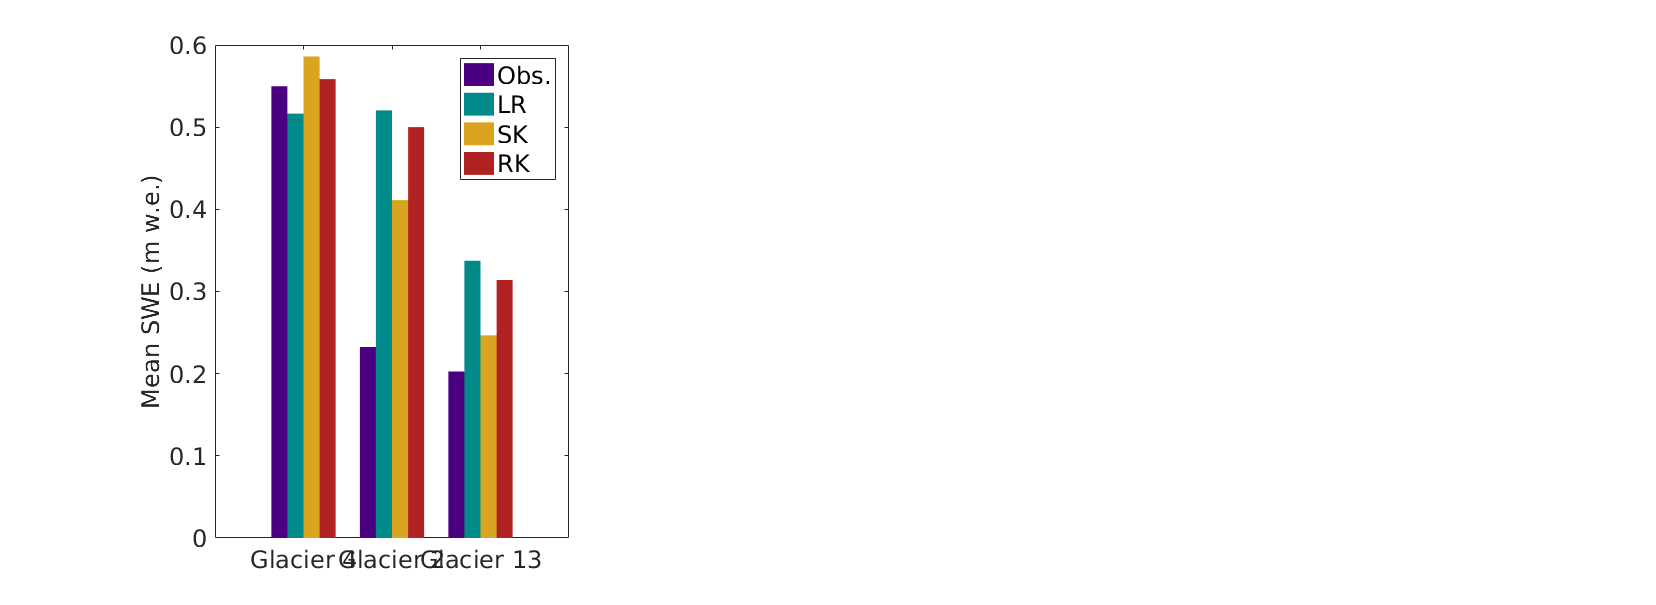
\includegraphics[width=1\textwidth]{InterpMethod_mean.png}}%
	\caption{Mean observed SWE and estimated winter balance using topographic regression, kriging, and regression kriging , averaged over density options.}
	\label{fig:InterpMethod_mean}
\end{figure}

For all glaciers, the topographic regression results in the lowest mean variance explained (Figure \ref{fig:InterpMethod_meanR2}). The mean correlation coefficients for kriging and regression kriging are similar for all glaciers, with regression kriging being slightly lower than kriging. Variance explained on Glacier 4 is consistently the lowest, indicating that observed SWE values are highly variable. The converse is seen on Glacier 2, where correlation coefficients are consistently high regardless of the interpolation method.

\begin{figure}
	\makebox[\textwidth][c]{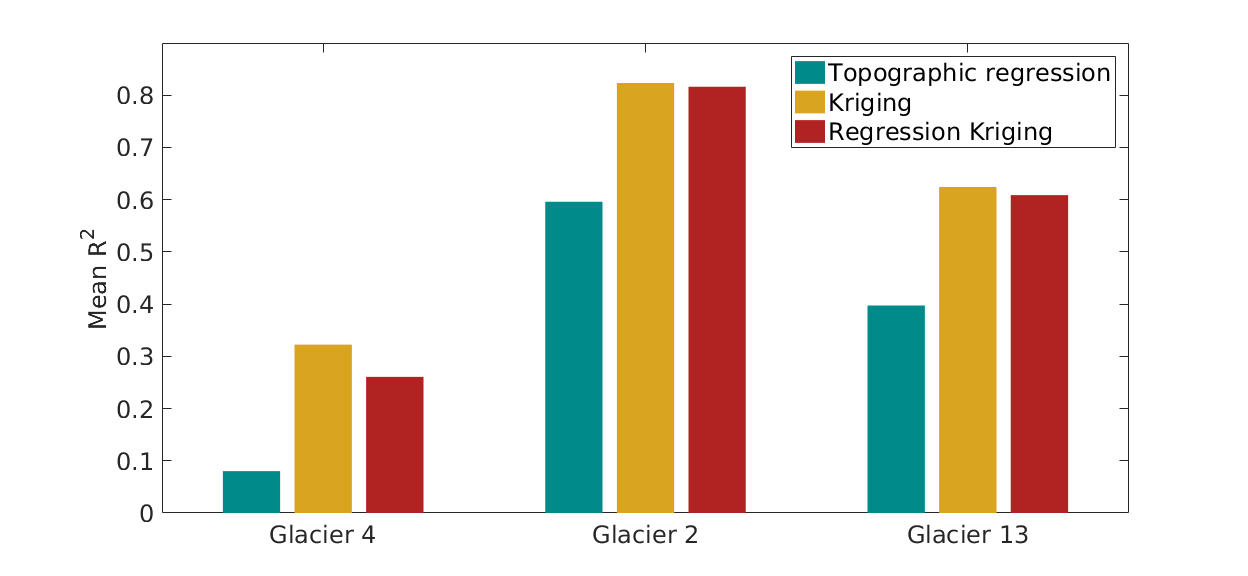
\includegraphics[width=1\textwidth]{InterpMethod_meanR2.png}}%
	\caption{Mean correlation coefficient (R$^2$) between observed SWE and estimated winter balance using topographic regression, kriging, and regression kriging at sampling locations, averaged over all density options.}
	\label{fig:InterpMethod_meanR2}
\end{figure}

The choice of density interpolation method generally does not affect the mean SWE value and their relative magnitudes (Figure \ref{fig:InterpMethod_allopts}). The main exception to this is that of kriging interpolation on Glacier 2, where a difference of almost 0.25 m w.e. exists between F3 and F4. The F3 option uses a linear regression between Federal Sampler-derived density and elevation to interpolate density values. There is a positive relationship (Figure ??), which means that the elevation gradient in SWE is increased, resulting in higher SWE point measurements in the accumulation area. This is turn increases the kriging estimate for the accumulation area beyond these points and raises the mean SWE. Again, it is clear that kriging is sensitive to individual measurement in sparsely sampled areas. It is surprising that the R$^2$ value for both these options is similar and high (Figure \ref{fig:InterpMethod_alloptsR2}), indicating that both estimates of winter balance are equally good. 

Regression kriging and kriging outperform topographic regression in prediciting SWE at measurement locations (Figure \ref{fig:InterpMethod_alloptsR2}). The correlation coefficient is similar for all density options on Glaciers 2 and 13. In all cases, R$^2$ values are highest for kriging and slightly lower for regression kriging (c.f. S3 on Glacier 13). However, the relative magnitude of R$^2$ values on Glacier 4 differs between kriging and regression kriging when different density options are chosen.  ??Reason??

topo vs kriging
topo -> spatial and temporal transferability (minimal/reference data needed), physically based so extrapolation less crazy)
kriging -> temporal transferability but not spatial, sensitive to sparsely sampled areas (our case, we have locally density and globally spare so lar extrapolation problems)


\begin{landscape}
\begin{figure}
	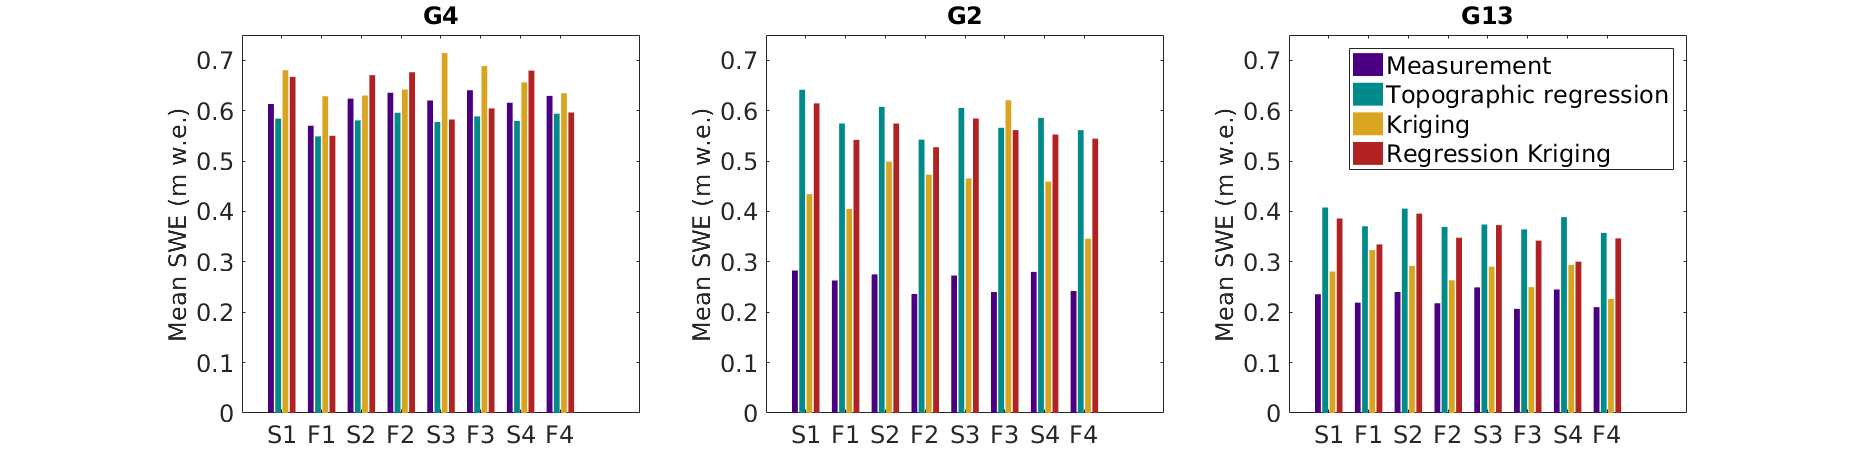
\includegraphics[height=0.38\textwidth]{InterpMethod_allopts.png}%
	\caption{Mean SWE and mean estimated winter balance using topographic regression, kriging, and regression kriging.}
	\label{fig:InterpMethod_allopts}
\end{figure}

\begin{figure}
	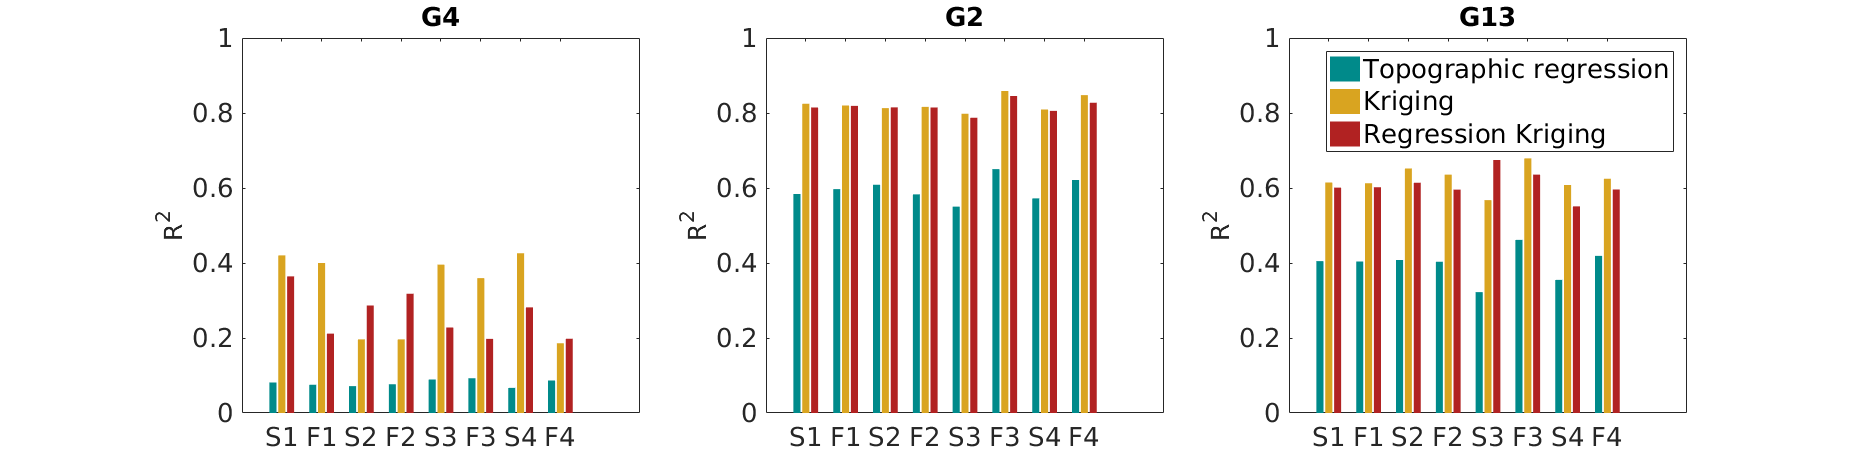
\includegraphics[height=0.38\textwidth]{InterpMethod_alloptsR2.png}%
	\caption{Correlation coefficient (R$^2$) between observed SWE and mean estimated winter balance using topographic regression, kriging, and regression kriging at sampling locations.}
	\label{fig:InterpMethod_alloptsR2}
\end{figure}
\end{landscape}
%%%%%%%%%%%%%%%%%%%%%
\bibliography{/home/glaciology1/Documents/MastersDocuments/MastersLit}
\bibliographystyle{igs}
%%%%%%%%%%%%%%%%%%%%%

\section{APPENDIX - Kriging software}
\label{app:KrigingMethods}
Kriging is executed using the DiceKriging package in R \citep{Roustant2012}. The author-written Matlab function \texttt{KrigingR()} moves SWE data to R and then uses DiceKriging to find the estimated kriged surface, the upper and lower confidence intervals, the cross-validated (leave-one-out) estimates of SWE, as well as parameters that describe the kriging model fit (nugget, maximum log likelihood and mean constant). Input parameters of  \texttt{KrigingR()} are the snow data (e.g. SWE values), locations of measurements, and the name of the relevant glacier. The function follows these steps:
\begin{enumerate}
\item The working directory is changed to the `Kriging' folder
\item The DiceKriging.R script is run
	\begin{enumerate}
	\item The function \texttt{km()} estimates the best fit kriging model with a constant mean using the Mat\'ern $\nu = 3/2$ covariance kernel. The maximum log likelihood, model intercept (mean) and nugget estimates from the model are then extracted. 
	\item Leave-one-out cross validation is then applied to estimated values using the built-in DiceKriging function \texttt{leaveOneOut.km()}.
	\item Surface prediction is then done for the entire glacier. First, a grid that replicates the glacier DEM is created (point spacing every 40 m to match the size of the DEM). Then, the built-in DiceKriging function \texttt{predict()} is used to predict the surface values at all grid locations. The predicted values, as well as the upper and lower 95\% confidence intervals are returned. 
	\item All returned values are then saved as a .mat file.
	\end{enumerate}
\item The .mat file is imported into Matlab and the data are organized into a structure. Cells outside of the glacier outlines are set to \texttt{NaN} and negative SWE values are set to zero. The final data are then output from the Matlab function. 
\end{enumerate}


\end{document} 